% (e) Analýza a návrh implementace produktu (včetně diskuse různých alternativ a volby implementačního prostředí).

\chapter{Analýza a návrh implementace}
% Analýza a návrh implementace (včetně diskuse různých alternativ a volby implementačního prostředí).
% Detailní popis uživatele a jeho potřeb.
% Analýzu odkázat na komparativní test.
% Návrh odkázat na low fidelity test.
% V analýze neprezentovat finální řešení ale dopodrobna celý proces.

% TODO kolik času bylo věnováno

Analýza s návrhem probíhaly nezávisle na dvou místech -- po krátké analýze celku a určení vzájemných komunikačních rozhraní byly provedeny analýza s návrhem serverové aplikace a až po jejím dokončení začaly analýza s návrhem mobilní aplikace. V průběhu času jsem se k analýze a návrhu ještě několikrát vrátil a vylepšil / rozšířil to, co se ne vždy na poprvé povedlo.

Analýza se skládala z identifikace potřeb uživatelů, vytvoření případů užití, ze kterých byly odvozeny funkční požadavky, ke kterým byly doplněny nefunkční požadavky. Poté byl vytvořen návrh řešení, zapracován návrh bezpečnosti a celý koncept byl podložen návrhem nasazení. Nakonec byly voleny technologie.

\section{Serverová aplikace}
Začal jsem pracovat nejprve na serverové aplikaci -- jednak na ní měla být ta mobilní závislá (sama na žádné jiné části práce závislá není) a také má užší vazbu ke zpracovávané doméně.


\subsection{Potřeby uživatelů}
\label{sec:server:needs}
Tato část se věnuje potřebám uživatelů serverové aplikace, zejména uživatelů rozhraní, přes které poskytuje informace. Potřeb je mnoho -- proto zde uvedu pouze reprezentativní vzorek.

\subsubsection{Potřeba zjistit informaci}
Potřeba zjistit informaci je základní potřebou, kvůli které se mají uživatelé obracet na systém. Tato potřeba může vzniknout z velikého množství příčin -- od hledání informací spjatých s průchodem studiem, až například po zjišťování jídelního lístku v menze.

\subsubsection{Potřeba ověřit informaci}
Často je cílová skupina uživatelů v situaci, kdy má požadovanou informaci, není si jí ale jistá a potřebuje ji ověřit / vyvrátit. Bez jistoty pravdivosti informace je její hodnota podstatně nižší.

\subsubsection{Potřeba ověřených informací}
Velmi podstatnou potřebou je potřeba ověřených informací. Ačkoliv je název velmi podobný té předchozí, jedná se o dvě diametrálně odlišné potřeby, předchozí se bez naplnění této neobejde. Jakmile jsou informace poskytovány, je nutné, aby byly ověřené -- pravdivé.

\subsubsection{Potřeba aktuálních informací}
Potřeba aktuálních informací opět souvisí s již zmíněnými potřebami -- sebepravdivější jídelní lístek z předchozího dne mi při výběru dnešního oběda bohužel moc nepomůže.

\subsubsection{Potřeba kompletních informací}
Někdy nestačí jen pravdivé a aktuální informace, naopak vědomí záruky pravdivosti a aktuálnosti může i uškodit -- pokud totiž informace nejsou kompletní, může dojít k jejich misinterpretaci a pod vlivem záruk nedojde ke kritickému posouzení. Proto je zde i potřeba kompletních informací.

\subsubsection{Potřeba nalézt, co nehledám}
Na první pohled tato potřeba nedává smysl, v praxi se ale často vyskytují informace, které bychom měli znát a o jejich existenci nemáme ani ponětí. Je proto důležité ve vhodné chvíli sdělit i nepožadované informace, které jsou s velkou pravděpodobností pro adresáta důležité.


\subsection{Případy užití}
Případy užití (\textit{use cases}) jsou takové sekvence kroků, které reprezentují danou činnost prováděnou aktérem na systému a vedou od jejího zahájení až po naplnění.

V serverové aplikaci byli identifikováni celkem čtyři hlavní aktéři:
\begin{itemize}
 \item Uživatel -- student / softwarová komponenta (\textit{mobilní aplikace}).
 \item Správce -- administrativní pracovník fakulty.
 \item Plánovač -- softwarová komponenta.
 \item Zdroj -- server poskytující informace.
\end{itemize}
Roli správce by šlo dále dělit na specifičtější role, vzhledem k velmi nízkému rozsahu činností každé z nich (zpravidla jedna činnost), je vše zahrnuto pod tímto souhrnným názvem. Pod plánovačem je zase zahrnut aktér čas.

Uživatel se pouze dotazuje nad systémem a zjišťuje informace. Správce manuálně upravuje informace v systému, může vynutit aktualizaci a jinak spravuje systém. Plánovač automaticky obsluhuje aktualizace obsažených informací. Zdroj na vyžádání poskytne dané informace.

\subsubsection{UC-S-1: Vyžádání informací}
\subsubsection*{Aktéři:}
\begin{itemize}
 \item Uživatel.
\end{itemize}
\subsubsection*{Systém:}
\begin{itemize}
 \item Serverová aplikace.
\end{itemize}
\subsubsection*{Vstupní podmínky:}
\begin{itemize}
 \item Uživatel zná jazyk dotazovacího rozhraní systému.
 \item Uživatel má přístup k dotazovacímu rozhraní systému.
\end{itemize}
\subsubsection*{Hlavní scénář:}
\begin{itemize}
 \item Uživatel vytvoří dotaz.
 \item Uživatel odešle dotaz na rozhraní systému.
 \item Systém přijme dotaz.
 \item Systém zpracuje dotaz -- nalezne požadované informace.
 \item Systém odešle odpověď.
 \item Uživatel přijme odpověď.
 \item Uživatel zpracuje odpověď.
\end{itemize}
\subsubsection*{Alternativní scénáře:}
\begin{itemize}
 \item V případě neplatného dotazu je navráceno chybové hlášení.
 \item V případě chyby serveru je navráceno chybové hlášení.
\end{itemize}
\subsubsection*{Poznámky:}
\begin{itemize}
 \item V případě nenalezení informace je navrácena prázdná množina.
 \item Pokud je uživatelem softwarová komponenta, student ji obsluhující nemusí znát jazyk dotazovacího rozhraní -- může s komponentou komunikovat jiným způsobem a ta si požadavky do požadovaného jazyka převádět.
\end{itemize}

\subsubsection{UC-S-2: Aktualizace informací}
\subsubsection*{Aktéři:}
\begin{itemize}
 \item Plánovač.
 \item Zdroj.
\end{itemize}
\subsubsection*{Systém:}
\begin{itemize}
 \item Serverová aplikace.
\end{itemize}
\subsubsection*{Vstupní podmínky:}
\begin{itemize}
 \item Plánovač je řádně nastaven a spuštěn.
 \item Nastal čas aktualizace určitých informací.
\end{itemize}
\subsubsection*{Hlavní scénář:}
\begin{itemize}
 \item Plánovač zadá systému požadavek na aktualizaci určitých informací.
 \item Systém přijme požadavek.
 \item Systém dá zdroji požadavek na informace.
 \item Zdroj zpracuje požadavek a informace vrátí.
 \item Systém přijme informace.
 \item Systém zpracuje informace.
 \item Systém odešle plánovači potvrzení.
\end{itemize}
\subsubsection*{Alternativní scénáře:}
\begin{itemize}
 \item V případě chyby zdroje je navráceno chybové hlášení.
 \item V případě chyby zpracování informací je navráceno chybové hlášení.
\end{itemize}
\subsubsection*{Poznámky:}
\begin{itemize}
 \item Případné chyby jsou zaznamenány do logu.
 \item Aktualizaci může obdobným způsobem vynutit i správce.
 \item Zdrojů určitých informací může být i více a vzájemně se mohou doplňovat / ověřovat.
\end{itemize}

\subsubsection{UC-S-3: Správa informací}
\subsubsection*{Aktéři:}
\begin{itemize}
 \item Správce.
\end{itemize}
\subsubsection*{Systém:}
\begin{itemize}
 \item Serverová aplikace.
\end{itemize}
\subsubsection*{Vstupní podmínky:}
\begin{itemize}
 \item Správce má přístup do systému.
 \item Správce zná jazyk rozhraní správy systému.
\end{itemize}
\subsubsection*{Hlavní scénář:}
\begin{itemize}
 \item Správce vytvoří dotaz.
 \item Správce se připojí do systému.
 \item Správce odešle dotaz.
 \item Systém přijme dotaz.
 \item Systém zpracuje dotaz.
 \item Systém odešle odpověď.
 \item Správce přijme odpověď.
 \item Správce se odpojí ze systému.
 \item Správce zpracuje odpověď.
\end{itemize}
\subsubsection*{Poznámky:}
\begin{itemize}
 \item Případné chyby jsou zaznamenány do logu.
\end{itemize}


\subsection{Požadavky}
\subsubsection{Funkční požadavky}
Funkčními požadavky (\textit{functional requirements}) jsou myšleny takové požadavky, které jsou zaměřeny na jednotlivé funkcionality systému. Ne všechny požadavky budou nakonec implementovány, pouze jejich reprezentativní vzorek, dle kterého bude možné systém o ty ostatní rozšířit. Pro serverovou aplikaci mezi ně patří především:
\begin{enumerate}
 \item Aplikace bude čerpat informace o názvech budov z předstíraného adaptéru.\footnote{Vynecháno. Implementováno na straně \textit{mobilní aplikace}.}
 \item Aplikace bude čerpat informace o umístění budov z předstíraného adaptéru.\footnote{Vynecháno. Implementováno na straně \textit{mobilní aplikace}.}
 \item Aplikace bude čerpat informace o názvech místností z předstíraného adaptéru.\footnote{Vynecháno. Implementováno na straně \textit{mobilní aplikace}.}
 \item Aplikace bude čerpat informace o umístění místností z předstíraného adaptéru.\footnote{Vynecháno. Implementováno na straně \textit{mobilní aplikace}.}
 \item Aplikace bude čerpat seznam vyučujících z KOSapi (\url{http://kosapi.fit.cvut.cz/}).\footnote{Nahrazen zdroj za předstíraný adaptér -- žádný seznam vyučujících obsahující identifikátory (uživatelská jména) nebyl nalezen.}
 \item Aplikace bude čerpat seznam studentů z KOSapi.\footnote{Nahrazen zdroj za předstíraný adaptér -- z důvodů konzistence se zdrojem vyučujících.}
 \item Aplikace bude čerpat seznam neakademických pracovníků z předstíraného adaptéru.
 \item Aplikace bude čerpat informace o rozvrzích místností z KOSapi.\footnote{Vynecháno -- projektu KOSapi nebyl dosud umožněn přístup do komponenty studia. Implementováno na straně \textit{mobilní aplikace}.}
 \item Aplikace bude čerpat informace o rozvrzích vyučujících z KOSapi.\footnote{Vynecháno -- projektu KOSapi nebyl dosud umožněn přístup do komponenty studia. Implementováno na straně \textit{mobilní aplikace}.}
 \item Aplikace bude čerpat informace o kancelářích vyučujících z Usermap ČVUT (\url{http://usermap.cvut.cz/}).
 \item Aplikace bude čerpat informace o kontaktech vyučujících z Usermap ČVUT.
 \item Aplikace bude čerpat informace o rozvrzích studentů z KOSapi.\footnote{Nahrazen zdroj za libovolný zdroj ve formátu iCalendar -- projektu KOSapi nebyl dosud umožněn přístup do komponenty studia.}
 \item Aplikace bude čerpat informace o kontaktech studentů z Usermap ČVUT.
 \item Aplikace bude čerpat informace o kancelářích neakademických pracovníků z Usermap ČVUT.
 \item Aplikace bude čerpat informace o kontaktech neakademických pracovníků z Usermap ČVUT.
 \item Aplikace bude čerpat informace o akcích \glsname{CVUT} z Kalendáře akcí ČVUT (\url{http://akce.cvut.cz/}).
 \item Aplikace bude čerpat informace o harmonogramu akademického roku z předstíraného adaptéru (na základě \url{http://fit.cvut.cz/}).\footnote{Vynecháno. Implementováno na straně \textit{mobilní aplikace}.}
 \item Aplikace bude čerpat informace o datech \glsname{MAR} budovy T9.\footnote{Jednání o udělení přístupu nedopadla -- vyskytly se blíže nespecifikované technické komplikace na straně technickoprovozních služeb Fakulty architektury.}
 \item Aplikace bude čerpat informace o datech \glsname{MAR} kolejí Orlík.\footnote{Vynecháno. Implementováno na straně \textit{mobilní aplikace}.}
 \item Aplikace bude čerpat informace o datech \glsname{MAR} Masarykovy koleje.\footnote{Vynecháno -- data poskytována pouze pod licencí, kterou nebylo možné naplnit.}
 \item Aplikace bude čerpat informace o jídelníčcích menz z Jídelníčků menz (\url{http://agata.suz.cvut.cz/jidelnicky/}).
 \item Aplikace bude čerpat informace o otvírací době menz z Jídelníčků menz.\footnote{Vynecháno. Implementováno na straně \textit{mobilní aplikace}.}
 \item Aplikace bude čerpat informace o otvírací době \glsname{NTK} z Národní technické knihovny (\url{http://www.techlib.cz/}).\footnote{Vynecháno. Implementováno na straně \textit{mobilní aplikace}.}
 \item Aplikace bude čerpat informace o otvírací době Vydavatelství průkazů (\url{http://ke.customer.decent.cz/a021/mon/wc-mon.php?co=2}).\footnote{Vynecháno. Implementováno na straně \textit{mobilní aplikace}.}
 \item Aplikace bude čerpat informace o počtu lidí ve frontě ve Vydavatelství průkazů (\url{http://ke.customer.decent.cz/a021/mon/}).\footnote{Vynecháno.}
 \item Vytvořte / nalezněte / sestavte z dílčích částí ontologii reprezentující výše uvedené informace.
 \item Informace získané z jednotlivých zdrojů převádějte dle výše požadované ontologie pro další zpracování do \glsname{RDF}.
 \item Aplikace umožní automatické aktualizace informací.
 \item Aplikace umožní manuální aktualizace informací.
 \item Aplikace umožní manuální úpravy informací.
%  \item Aplikace bude logovat chyby.
 \item Aplikace bude ukládat sémantické informace do databáze.
 \item Aplikace umožní vykonávat dotazy nad uloženými daty.
\end{enumerate}

\subsubsection{Nefunkční požadavky}
Nefunkčními požadavky (\textit{non-functional requirements}) jsou myšleny takové požadavky, které jsou zaměřeny na dílo jako celek, nikoliv na jednotlivé funkcionality. Pro serverovou aplikaci mezi ně patří především:

\begin{enumerate}
 \item Aplikaci naprogramujte v jazyce JavaScript.
 \item Pro běh serveru využijte Node.js.
 \item Pro dotazování využijte dotazovací jazyk \glsname{SPARQL}.
 \item Sémantická data ukládejte do takového úložiště, aby nad ním bylo možné vykonávat dotazy přímo (případně přes nezávislého prostředníka) a nebylo nutné přistupovat přes vlastní aplikaci.
 \item Práce nemusí nutně obsáhnout celou zpracovávanou doménu, je ale žádané, aby kvalitně zpracovala hlavní scénáře využití a nebránila dalšímu rozšiřování.
 \item Zveřejněte aplikaci a její data pod svobodnými licencemi z rodin \glsname{GNU}, Creative Commons a kompatibilními, aby byl umožněn další rozvoj nezávislý na původním autorovi.
\end{enumerate}


\subsection{Návrh ontologie}
Tvorbě ontologie bylo věnováno velmi dlouhé období -- neměl jsem s tímto oborem předchozí zkušenosti a vytvoření kvalitní ontologie považuji jako nutný předpoklad pro následné pokračování -- na špatných základech nelze vybudovat kvalitní systém.

Zpočátku jsem vytvářel ontologii od základů vlastní, s přibývajícími zkušenostmi jsem si ale uvědomil, že to nebyl dobrý nápad -- ve světě sémantického webu je jednou z nejdůležitějších priorit vzájemná interoperabilita -- s každou novou ontologií je tak vzájemné mapování informací čím dál tím těžší. V té době jsem veškerou svou dosavadní práci zahodil a začal znovu.

Nejprve jsem se vrátil k výsledkům rešeršního zpracování ontologií a vybral z nich tu, která se mi zdála po v mezičase nabitých zkušenostech nejlepší -- \gls{AIISO}. Tato ontologie je již předurčená k využití s ontologiemi Participation, \gls{FOAF} a AIISO Roles. Ontologie jsou to již zaběhlé, takže problém s interoperabilitou pozbyl platnosti.

Dalším bodem zvratu bylo zjištění, jak složité může být nalezení styčných bodů mezi obecnou ontologií a konkrétní situací. Bylo třeba v některých případech nalézt další vhodné ontologie reprezentující doposud nepokryté oblasti, případně již použité ontologie rozšířit (zpravidla je použita licence Creative Commons, takže je rozšiřování možné). Příkladem může být reprezentace akcí \glsname{CVUT} -- žádná z použitých ontologií nemodeluje události. Abych se dodržel kurzu ve směru interoperability, bylo třeba nalézt vhodnou ontologii. Nabízelo se jich několik, nakonec byla použita \gls{LODE}, právě kvůli svému zastřešení obdobných ontologií.

Následuje seznam zvolených ontologií, pro specifické případy se ale počítá s jeho dalším rozšiřováním:
\begin{itemize}
 \item \Glsname{AIISO} (\url{http://purl.org/vocab/aiiso/schema}).
 \item Participation (\url{http://purl.org/vocab/participation/schema}).
 \item \Glsname{FOAF} (\url{http://xmlns.com/foaf/0.1/}).
 \item AIISO Roles (\url{http://purl.org/vocab/aiiso-roles/schema}).
 \item \Glsname{LODE} (\url{http://linkedevents.org/ontology/}).
 \item \Glsname{OWLTime} (\url{http://www.w3.org/TR/owl-time/}).
\end{itemize}


\subsection{Návrh architektury}
Nejprve byl vytvořen návrh architektury (\textit{architecture design}) aplikace, který byl později rozpracován do návrhu nasazení (\textit{deployment design}).

Identifikovány byly následující základní struktury systému:
\begin{itemize}
 \item \textit{Serverová aplikace.}
 \item Plánovač.
 \item Databáze.
 \item \glsname{SPARQL} endpoint.
\end{itemize}
Pod pojmem \textit{serverová aplikace} se skrývá aplikace, která získává data přímo ze zdrojů, z nich vybírá informace, ty strukturuje a ukládá do databáze. Plánovač je reprezentován aplikací, která ve vhodné časy vyžádá na serveru aktualizaci informací. \glsname{SPARQL} endpoint je aplikace, která na požadavek v dotazovacím jazyku vrátí odpovídající data z databáze. Databáze je úložištěm informací.

Nasazení bylo nakonec navrženo, jak je vidět na obrázku \ref{fig:server:deployment}, umístěním všech prvků serverové aplikace na jediný server, který získává informace z prostředí Internetu a zároveň poskytuje informace uživatelům.
\begin{figure}[h]
 \centering
 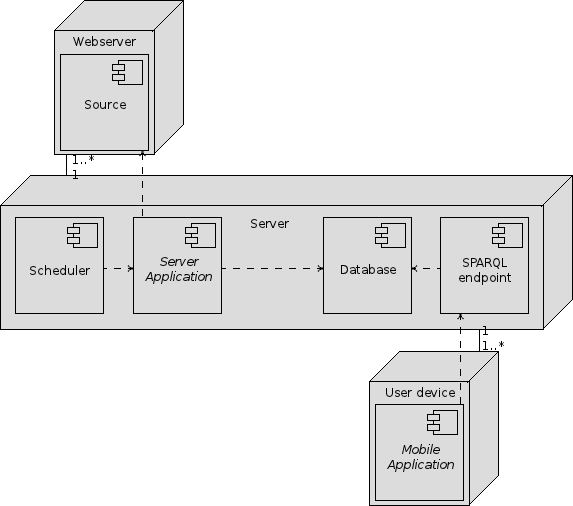
\includegraphics{./figures/deployment-s.png}
 % deployment-s.png: 573x506 pixel, 112dpi, 13.00x11.48 cm, bb=0 0 368 325
 \caption{Diagram nasazení serverové aplikace}
 \label{fig:server:deployment}
\end{figure}


\subsection{Návrh řešení}
Návrh (\textit{design}) byl prováděn po rozvržení architektury a za přispění volby použitých technologií.

Pro tři ze čtyř dříve identifikovaných struktur systému jsem nalezl vhodné hotové řešení (viz část \ref{sec:server:technologies} na straně \pageref{sec:server:technologies}) -- plánovač je tvořen cronem, jako databáze je použita MongoDB a \glsname{SPARQL} endpoint poskytuje rdfstore. Zbývá tedy doimplementovat pouze \textit{serverovou aplikaci}.

Na obrázku \ref{fig:server:class} je znázorněn třídní diagram (\textit{class diagram}) reprezentující strukturu serverové aplikace. Metoda \textbf{process()} má za úkol stažení dat z patřičných zdrojů, jejich zpracování, převedení do sémantických grafů a uložení do databáze. V návrhu byl použit návrhový vzor strategie (\textit{strategy}).

\begin{figure}[h]
 \centering
 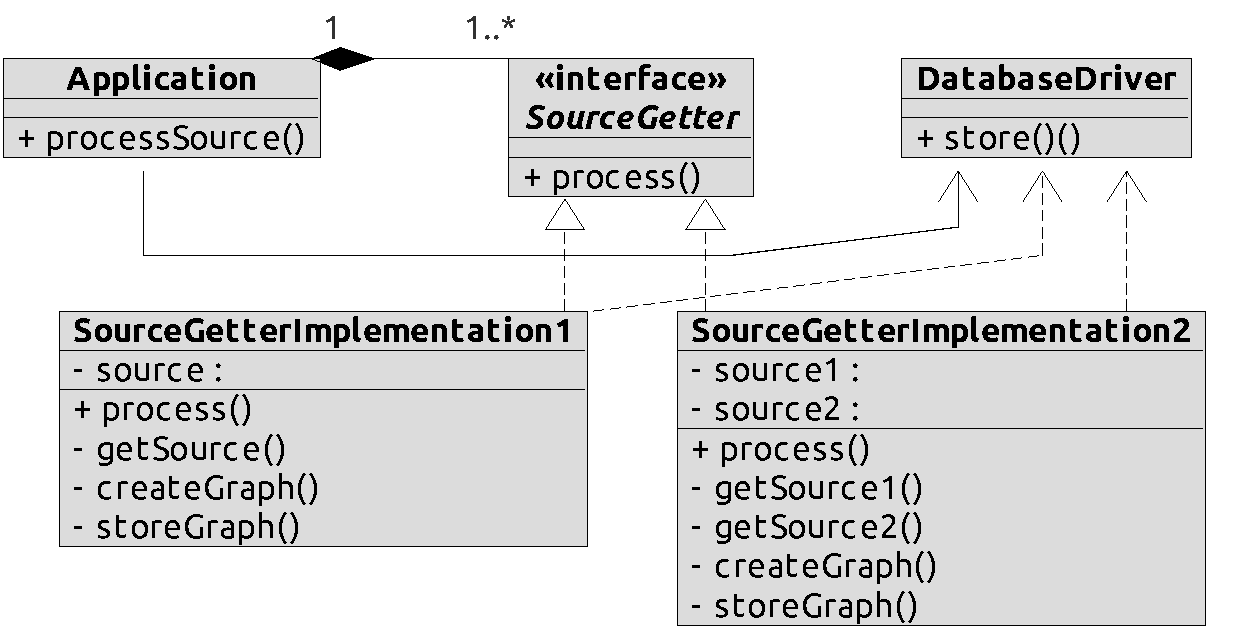
\includegraphics[width=11.47cm]{./figures/class-s.pdf}
 \caption{Třídní diagram serverové aplikace}
 % class-s.png: 429x190 (218) pixel, 95dpi, 11.47x5.08 cm, bb=0 0 325 144
 \label{fig:server:class}
\end{figure}



\subsection{Návrh bezpečnosti}
% \todo{Injekce kódu. Pouze povolené URL. Ošetření vstupů.}
Po zběžném návrhu aplikace byly modelovány hrozby. Nejprve jsem aplikaci dekomponoval na důvěryhodné a nedůvěryhodné komponenty systému a určil mezi nimi hranice důvěry. Poté jsem identifikoval hrozby. Nakonec byly identifikovány zranitelnosti. Vymodelované hrozby byly následně snižovány.

\subsubsection{Dekompozice}
Byly identifikovány následující komponenty (obdobné s těmi z návrhu architektury):
\begin{itemize}
 \item \textit{Serverová aplikace.}
 \item Plánovač.
 \item Databáze.
 \item \glsname{SPARQL} endpoint.
 \item Uživatel.
 \item Zdroj informací.
\end{itemize}
Plně důvěřovat můžu pouze serverové aplikaci a plánovači -- mají to být vlastní jednoduché aplikace. Dále lze do určité míry důvěřovat databázi a \glsname{SPARQL} endpointu -- aplikace budou provozovány pod vlastní správou. Zdroje informací a uživatelské aplikace jsou naopak nedůvěryhodné -- jsou plně v režii třetích stran. Hranice důvěry jsou nicméně mezi všemi komponentami.

\subsubsection{Identifikace hrozeb}
U komponenty \emph{serverová aplikace} byly identifikovány následující hrozby:
\begin{itemize}
 \item Podvržení nepravdivých dat.
 \item Přetížení komponenty velkým počtem požadavků.
\end{itemize}
U komponenty \emph{databáze} byly identifikovány následující hrozby:
\begin{itemize}
 \item Přetížení komponenty velkým počtem požadavků.
 \item Podvržení nepravdivých dat.
\end{itemize}
U komponenty \emph{\glsname{SPARQL} endpoint} byly identifikovány následující hrozby:
\begin{itemize}
 \item Přetížení komponenty velkým počtem požadavků.
 \item Podvržení identity uživatele.
 \item Únik informací.
\end{itemize}
U komponenty \emph{plánovač} nebyly identifikovány, vzhledem k jednoúčelovému zaměření, žádné hrozby.

\subsubsection{Identifikace zranitelností}
Všechny výše uvedené hrozby mohou vyústit ve zranitelnosti, nejvyšší prioritu mají ty nejpravděpodobnější -- na hranicích důvěry směrem k uživatelům a zdrojům dat. S hrozbou můžeme naložit následovně:
\begin{itemize}
 \item Ponechat v programu.
 \item Odstranit problém.
 \item Odstranit hrozbu.
\end{itemize}
Preferovaná je zpravidla poslední možnost.

\subsubsection{Důsledky}
\begin{itemize}
 \item Je třeba důsledně ošetřovat vstupy (aby nedošlo k uložení škodlivých dat do databáze, aby na \glsname{SPARQL} endpointu nebyly prováděny jiné operace, než dotazovací\dots).
 \item Je třeba vše ve výchozím nastavení vše zakázat a k potřebným úkonům udělit výjimky (pouze dotazy nad \glsname{SPARQL} endpointem, přístup jen k některým zdrojům ze serverové aplikace\dots).
 \item Je třeba zamezit odepření služeb (přetížením \glsname{SPARQL} endpointu, zahlcením databáze\dots).
\end{itemize}


\subsection{Použité technologie}
\label{sec:server:technologies}
Mnoho použitých technologií bylo dáno zadáním práce, byl mi tak do značné míry usnadněn jejich výběr. Na druhou stranu nejsou některé z technologií příliš ověřené, zdokumentované a neexistují k nim příklady, takže by často bývala práce s jinými snazší.

Celá serverová aplikace je napsána v JavaScriptu, zprovozněna na Node.js, datovým úložištěm se stalo MongoDB.

\subsubsection{JavaScript}
Využití JavaScriptu bylo, pro svoje pravděpodobné vzrůstající nasazení v budoucnosti a své specifické vlastnosti, dáno jako nefunkční požadavek.

\subsubsection{Node.js}
Node.js (\url{http://nodejs.org/}) je platforma postavená nad běhovým prostředím JavaScriptu z webového prohlížeče Google Chrome. Slouží ke tvorbě rychlých, škálovatelných síťových aplikací. Node.js využívá událostmi řízený neblokovací I/O model, který ho činí nenáročným a efektivním, vhodným pro datově náročné \textit{real-timové} aplikace běžící v distribuovaném prostředí \cite{Node}.

Použití Node.js bylo vynuceno nefunkčním požadavkem, jedná se ale o velmi cennou zkušenost -- je novou technologií a ačkoliv je jeho dokumentace na slušné úrovni, není zatím vytvořena dostatečně velká báze příkladů a nejlepších praktik.\footnote{Takže jsem se k dobrým praktikám musel postupně propracovat a při té příležitosti se toho hodně naučil. Navíc, zdá se, se budou nabité vědomosti v budoucnu hodit.}

\subsubsection{MongoDB}
MongoDB (\url{http://www.mongodb.org/}) je škálovatelnou, vysoce výkonnou, otevřenou NoSQL databází napsanou v C++ \cite{Mongo}.

Databázi jsem volil z dalších sémantických / NoSQL databází (zaměření dáno požadavkem na použití nových inovativních technologií), zvažovány byly mimo jiné i CouchDB (\url{http://couchdb.apache.org/}), Neo4j (\url{http://neo4j.org/}) a Openlink Virtuoso (\url{http://virtuoso.openlinksw.com/}).

Poslední jmenovaná databáze byla na základě předchozích zkušeností vybrána nejdříve, později se ale ukázalo, že jsou její správa i obsluha pro konkrétní použití těžkopádné, takže jsem nakonec přešel k podstatně vhodnější databázi, MongoDB, kterou lze navíc snadno využít v kombinaci s JavaScriptovým \glsname{RDF} úložištěm rdfstore (viz část \ref{sec:rdfstore}).

\subsubsection{cron}
Cron je démonem vykonávajícím naplánované úlohy. Název neoznačuje konkrétní implementaci, ale používá se pro označení programu splňujícího určité specifikace (jak je u Unixových nástrojů zvykem). Byla vybrána implementace, jejímž autorem je Paul Vixie -- jedná se o verzi využitou například v \glsname{GNU}/Linuxu a \glsname{BSD} (odkud pochází).

Cron byl vybrán pro svou vhodnost pro daný účel, plánovat, a pro svoji prověřenost.

\subsubsection*{ }
Celé prostředí serverové aplikace je umístěno v serverové edici \glsname{GNU}/linuxové distribuce Ubuntu (\url{http://www.ubuntu.com/}) a ta je pro snadnou přenositelnost nainstalována do kontejneru virtuálního stroje virtualizačního řešení VirtualBox (\url{http://www.virtualbox.org/}). Technologie byly vybrány na základě výborných předchozích zkušeností.

\subsection{Použité knihovny}
Mimo standardního JavaScriptu lze v Node.js využívat i specifická rozšíření a množství modulů třetích stran. Z těch jsem po zvážení z různých příčin využil:

\subsubsection{node-date-utils}
Node-date-utils (\url{https://github.com/JerrySievert/node-date-utils}) je mikro frameworkem doplňujícím funkcionalitu JavaScriptového objektu Date. Nástroj byl vybrán z potřeby snadno formátovat čas.

Zvažováno bylo i použití obdobného nástroje node-dateformat (\url{https://github.com/felixge/node-dateformat}), ten je ale svou nabídkou funkcionalit pro projekt méně vhodný. Oba moduly jsou stále ve vývoji.

\subsubsection{express}
Express (\url{http://expressjs.com/}) je renomovaným frameworkem pro tvorbu webových aplikací. Je založený na middleware frameworku connect (\url{http://www.senchalabs.org/connect/}).

Express byl vybrán jako ověřené řešení pro vytvoření struktury webové aplikace -- nejenže v sobě zahrnuje mnoho dobrých praktik, ke kterým bych jen stěží došel vlastním zkoumáním, ale přináší zároveň i markantní zjednodušení struktury kódu aplikace.

\subsubsection{node-icalendar}
Node-icalendar (\url{https://github.com/tritech/node-icalendar}) je knihovnou pro práci s formátem iCalendar. Je stále ve vývoji, nicméně množina poskytovaných funkcionalit je pro tuto práci dostatečná.

Zvažovány byly i další knihovny, například node-ical (\url{https://github.com/peterbraden/node-ical}), ty ale neimplementují dostatek funkcionality potřebné pro tvorbu aplikace.

\subsubsection{node-iconv}
Node-iconv (\url{https://github.com/bnoordhuis/node-iconv}) je knihovnou pro obsluhu systémového příkazu iconv sloužícího k převádění kódování. Knihovna byla vybrána pro bezpečnou implementaci převodu kódování.

\subsubsection{node-jquery}
Node-jquery (\url{https://github.com/coolaj86/node-jquery}) je \textit{wrapperem} umožňujícím využít renomovanou JavaScriptovou knihovnu jQuery (\url{http://jquery.com/}) v prostředí Node.js.

jQuery bylo vybráno pro usnadnění zpracování externích zdrojů dat -- nabízí prověřené způsoby selekce, traverzování a manipulace s \glsname{DOM}.

Node-jquery interně využívá modul jsdom (\url{https://github.com/tmpvar/jsdom}), který mu poskytuje JavaScriptovou implementaci \glsname{DOM}.

\subsubsection{rdfstore}
\label{sec:rdfstore}
Rdfstore (\url{https://github.com/antoniogarrote/rdfstore-js}) je JavaScriptovou implementací \glsname{RDF} grafového úložiště s podporou pro \glsname{SPARQL}. Data mohou být (a v implementaci \glsname{DP} jsou) persistentně ukládána prostřednictvím Node.js modulu-ovladače node-mongodb (\url{https://github.com/christkv/node-mongodb-native}) do NoSQL databáze MongoDB (\url{http://www.mongodb.org/}). Modul je stále ve vývoji.

Právě pro implementaci manipulace s \glsname{RDF}, grafové úložiště a podporu pro \glsname{SPARQL} byl rdfstore vybrán jako základ pro \glsname{SPARQL} endpoint a důležitá součást \textit{serverové aplikace}.

% \subsubsection{node-soap}
%  (\url{https://github.com/milewise/node-soap}) -- \todo{Pouze pokud se objeví podpora poskytnutého WSDL.}


\subsection{Použité nástroje}
\label{sec:server:tools}
Pro tvorbu serverové aplikace byly vybrány následující nástroje:
\subsubsection{Kate}
\label{sec:server:tools:kate}
Pro implementaci serverové aplikace, stejně jako pro mnoho dalších činností, byl vybrán textový editor \glsname{Kate} (\url{http://kate-editor.org/}) z prostředí \glsname{GNU}/Linuxového desktopového prostředí \glsname{KDE}. \glsname{Kate} nabízí zvýrazňování syntaxe všech v diplomové práci použitých formátů, poskytuje velmi užitečnou práci s regulárními výrazy, umožňuje pracovat s mnoha soubory najednou a, co je asi nejpodstatnější, plně se integruje do (mnou používaného) \glsname{KDE}, takže ním například lze prostřednictvím \gls{KIO} transparentně pracovat se vzdálenými soubory. \glsname{Kate} neumožňuje automatické doplňování kódu, nabízí ale již použitá slova kdekoliv v dokumentu, což je vlastnost v mnoha ohledech srovnatelná. \Glsname{Kate} byl zvolen i na základě velice kladných zkušeností pro vytvoření zdrojového kódu a konfiguračních souborů.

\subsubsection{Kompare}
\label{sec:server:tools:kompare}
Pro případ potřeby důkladného porovnání souborů byl vybrán Kompare (\url{http://www.caffeinated.me.uk/kompare/}). Nástroj umožňuje velmi přehledně porovnat mimo jednotlivých souborů i celé jejich adresáře. Kompare neporovnává soubory sám, ale je nadstavbou nad konzolovou aplikací diff či obdobnou. Mimo již popsaných vlastností byl Kompare vybrán i pro svou integraci s \glsname{KDE}.

\subsubsection{Webové prohlížeče}
Pro průzkum zdrojů a jejich struktur byly zvoleny internetové prohlížeče a jejich rozšíření:
\begin{itemize}
 \item Mozilla Firefox (\url{http://www.mozilla.org/firefox}) + Firebug (\url{http://getfirebug.com/}).
 \item Chromium (\url{http://chromium.org/}).
\end{itemize}

\subsubsection{Protégé}
Pro průzkum a práci s ontologiemi byl zvolen editor Protégé (\url{http://protege.stanford.edu/}). Rozhodnutí bylo učiněno pro nabídku funkcionalit a předchozí zkušenosti.

\subsubsection{curl}
Konzolový nástroj curl z projektu \glsname{cURL} (\url{http://curl.haxx.se/}) byl zvolen pro snadnou kontrolu cizích zdrojů i vlastní vytvářené aplikace.

\subsubsection{Git}
\label{sec:server:tools:git}
Pro správu verzí práce byl zvolen nástroj Git (\url{http://git\-scm.com/}), čímž má být zajištěné pohodlné zálohování, jak ve smyslu možnosti návratu k některé z minulých verzí, tak i ve smyslu vzdáleného duplikování na serveru GitHub (\url{http://github.com/}). Pozitivním vedlejším efektem tohoto přístupu je možnost sledování vývoje prostřednictvím veřejného repozitáře.


\section{Mobilní aplikace}
Mobilní aplikace má sloužit studentům jako průvodce a měla by spolupracovat se serverovou aplikací. Vzhledem k této závislosti je třeba ji realizovat až po té serverové, ovšem analýza s návrhem by měly probíhat kvůli vzájemné spolupráci v některých fázích souběžně.

\subsection{Potřeby uživatelů}
Následující část se věnuje identifikaci základních potřeb potenciálních uživatelů aplikace, které by jim mohla / měla naplnit -- na jejich základě totiž budou hledány uživatelské scénáře a požadavky.

\subsubsection{Potřeba informací}
Pod tuto potřebu shrnuji všechny potřeby nalezené u serverové aplikace (viz část \ref{sec:server:needs} na straně \pageref{sec:server:needs}). Jsou to:
\begin{itemize}
 \item Potřeba zjistit informaci.
 \item Potřeba ověřit informaci.
 \item Potřeba ověřených informací.
 \item Potřeba aktuálních informací.
 \item Potřeba kompletních informací.
 \item Potřeba nalézt, co nehledám.
\end{itemize}
Zejména naplnění poslední potřeby -- předložit informaci, o kterou člověk sice nepožádal, ale udělal by to, kdyby ho to bylo napadlo -- je od průvodce vítané.

\subsubsection{Potřeba uživatelské přívětivosti}
Vzhledem k předpokládanému využití mobilní aplikace podstatně méně pokročilými uživateli, oproti serverové, je vhodné, aby tomu byla uzpůsobena. Cílová skupina navíc zpravidla není ochotná číst dlouhé návody a je tak třeba, aby byla aplikace použitelná sama o sobě.

\subsubsection{Potřeba určit cílovou pozici}
Jedna z nejdůležitějších potřeb, které by měl průvodce naplnit, je potřeba určit cílovou pozici. Může to být například:
\begin{itemize}
 \item Budova, učebna, kancelář, knihovna\dots
 \item Menza, hospoda, občerstvení, nápojový automat\dots
 \item Pitná voda, toalety, sprchy\dots
 \item Výtah, schodiště, nájezd pro kočárek\dots
 \item Vchod, únikový východ, hasící přístroj\dots
 \item Bankomat, zastávka \glsname{MHD}, parkoviště\dots
 \item Informace, vrátnice, šatna, údržba\dots
\end{itemize}
Ačkoliv jsou v seznamu uvedené pozice rozděleny do určitých logických celků, je důležité si povšimnout, že existují i jiná jejich, v některých ohledech důležitější, uspořádání:
\begin{itemize}
 \item Dle jednoznačnosti místa -- místnost s jasně daným názvem je oproti libovolnému schodišti jediná.
 \item Dle jednoznačnosti identifikátoru -- stejná místnost může být vyhledána na základě různých kritérií (název, následující výuka, popis).
 \item Dle frekvence hledání -- přednáškové místnosti jsou vyhledávány podstatně častěji, než hasící přístroje.
 \item Dle kritéria priority -- vzdálenější menza může mít vyšší prioritu na základě lepší kuchyně, zatímco sebelepší nápojový automat může mít kvůli své větší vzdálenosti prioritu nižší.
\end{itemize}
Pro úplnost ještě uvádím seznam informací vedoucích k určení cílové pozice:
\begin{itemize}
\item Označení místnosti, budovy\dots (T9:349, TK\dots).
\item Název místnosti, budovy\dots (Gočár, Národní technická knihovna\dots).
\item Neoficiální název místnosti, budovy\dots (Bouračka, Modrá menza\dots).
\item Jméno, pokud hledáme kancelář vyučujícího nebo neakademického pracovníka.
\item Rozvrh, pokud hledáme místo další výuky nebo zkoušky.
\item Zeměpisné souřadnice.
\item Poloha všech míst, které přicházejí v úvahu (toalety, bankomaty\dots) -- hledající si vybere.
\item Předchozí bod a navíc přibližná aktuální poloha -- lze určit nejbližší.
\end{itemize}
Přehledy rozšiřují poznatky získané při tvorbě bakalářské práce \cite{Bakalarka}.

\subsubsection{Potřeba určit aktuální pozici}
Zvláště, pokud máme mapu nebo jsme v jiné situaci, kdy víme, kam jít, vyvstává potřeba určit aktuální pozici -- bez té totiž nelze určit směr, vzdálenost, a v případě, že hledáme nejbližší místo daného typu, ani cíl cesty.

\subsubsection{Potřeba nezávislosti}
Cílová skupina má díky specifickému životnímu stylu silnou potřebu nezávislosti v mnoha oblastech -- pokud jim má být poskytnu aplikace, ani ta je nesmí příliš omezovat -- je proto vhodné, aby se jednalo o aplikaci mobilní a aby umožňovala offline provoz, jinak hrozí nemožnost jejího využití v situacích jako je cesta do školy nebo přítomnost na některém z mnoha signálem nepokrytých míst budovy T9.

% \subsection{Potřeba multiplatformní aplikace}
% 
% \subsubsection{Potřeby návštěvníků na aplikaci}
% \todo{externí přednášející, dny otevřených dveří, partnerky studentů...}


\subsection{Případy užití}
U případů užití (\textit{use cases}) mobilní aplikace byli identifikováni jediní dva aktéři:
\begin{itemize}
 \item Uživatel -- student.
 \item Server -- \glsname{SPARQL} endpoint.
\end{itemize}
Dále byly identifikovány tři hlavní případy užití:
\begin{itemize}
 \item Získání určité (textové) informace.
 \item Vyhledání (mapové) pozice.
 \item Vykonání \glsname{SPARQL} dotazu.
\end{itemize}

\subsubsection{UC-M-1: Získání jídelníčku}
\subsubsection*{Aktéři:}
\begin{itemize}
 \item Uživatel.
 \item Server.
\end{itemize}
\subsubsection*{Systém:}
\begin{itemize}
 \item Mobilní aplikace.
\end{itemize}
\subsubsection*{Vstupní podmínky:}
\begin{itemize}
 \item Uživatel se nachází na patřičném místě systému.
 \item Systém má připojení k serveru.
\end{itemize}
\subsubsection*{Hlavní scénář:}
\begin{itemize}
 \item Uživatel nalezne akci získání jídelníčku.
 \item Uživatel dá požadavek na získání jídelníčku.
 \item Systém odešle požadavek na server.
 \item Server zpracuje požadavek a odešle odpověď.
 \item Systém přijme odpověď
 \item Systém zpracuje odpověď.
 \item Systém vizualizuje jídelníček.
\end{itemize}
\subsubsection*{Alternativní scénáře:}
\begin{itemize}
 \item V případě chyby připojení je navráceno chybové hlášení.
 \item V případě neexistence jídelníčku je navráceno oznámení.
\end{itemize}
\subsubsection*{Poznámky:}
\begin{itemize}
 \item Místo získávání jídelníčku může být prováděna libovolná obdobná činnost.
 \item Pro některé obdobné informace nemusí být vyžadováno připojení k serveru, záleží na době jejich platnosti.
\end{itemize}

\subsubsection{UC-M-2: Vyhledání občerstvení}
\subsubsection*{Aktéři:}
\begin{itemize}
 \item Uživatel.
\end{itemize}
\subsubsection*{Systém:}
\begin{itemize}
 \item Mobilní aplikace.
\end{itemize}
\subsubsection*{Vstupní podmínky:}
\begin{itemize}
 \item Uživatel se nachází na patřičném místě systému.
\end{itemize}
\subsubsection*{Hlavní scénář:}
\begin{itemize}
 \item Uživatel zadá do vyhledávacího pole požadavek na občerstvení.
 \item Uživatel potvrdí vyhledávání.
 \item Systém vyhledá všechna občerstvení.
 \item Systém vizualizuje nalezená občerstvení.
 \item Uživatel zadá požadavek na zobrazení aktuální polohy.
 \item Systém určí uživatelovu polohu.
 \item Systém vizualizuje polohu.
 \item Uživatel si dle poskytnutých informací vybere občerstvení.
\end{itemize}
\subsubsection*{Alternativní scénáře:}
\begin{itemize}
 \item V případě neplatného dotazu je navráceno chybové hlášení.
 \item V případě chyby určování polohy je navráceno chybové hlášení.
 \item V případě výskytu mimo mapu je navráceno chybové hlášení.
\end{itemize}
\subsubsection*{Poznámky:}
\begin{itemize}
 \item Místo vyhledávání občerstvení mohou být vyhledávány i jiné pozice.
 \item U některých typů dotazů není nutné znát aktuální polohu.
 \item U některých typů dotazů je navrácena jediná pozice.
\end{itemize}

\subsubsection{UC-M-3: Vykonání SPARQL dotazu}
\subsubsection*{Aktéři:}
\begin{itemize}
 \item Uživatel.
 \item Server.
\end{itemize}
\subsubsection*{Systém:}
\begin{itemize}
 \item Mobilní aplikace.
\end{itemize}
\subsubsection*{Vstupní podmínky:}
\begin{itemize}
 \item Uživatel se nachází na patřičném místě systému.
 \item Uživatel zná dotazovací jazyk \glsname{SPARQL}.
 \item Systém má připojení k serveru.
\end{itemize}
\subsubsection*{Hlavní scénář:}
\begin{itemize}
 \item Uživatel vytvoří dotaz.
 \item Uživatel potvrdí dotaz.
 \item Systém odešle dotaz na server.
 \item Server zpracuje požadavek a odešle odpověď.
 \item Systém přijme odpověď
 \item Systém zpracuje odpověď.
 \item Systém vizualizuje odpověď.
\end{itemize}
\subsubsection*{Alternativní scénáře:}
\begin{itemize}
 \item V případě neplatného dotazu je navráceno chybové hlášení.
 \item V případě chyby připojení je navráceno chybové hlášení.
 \item V případě chyby serveru je navráceno chybové hlášení.
\end{itemize}
\subsubsection*{Poznámky:}
\begin{itemize}
 \item V případě nenalezení informace je navrácena prázdná množina.
\end{itemize}


\subsection{Požadavky}
\subsubsection{Funkční požadavky}
Funkčními požadavky (\textit{functional requirements}) jsou myšleny takové požadavky, které jsou zaměřeny na jednotlivé funkcionality. Pro mobilní aplikaci mezi ně patří především:

\begin{enumerate}
 \item Aplikace umožní zadat vlastní \glsname{SPARQL} dotaz. Ten se odešle na server, kde se zpracuje, a výsledek se navrátí uživateli.
 \item Aplikace bude získávat data předpřipravenými \glsname{SPARQL} dotazy.
 \item Aplikace dokáže na mapě vizualizovat budovy.
 \item Aplikace dokáže na mapě vizualizovat místnosti.
 \item Aplikace dokáže na mapě vizualizovat body zájmu.
 \item Aplikace umožní určení aktuální pozice a její předání dalšímu zpracování.
 \item Aplikace dokáže na mapě vizualizovat polohu uživatele.
 \item Aplikace bude poskytovat nápovědu pro snazší použití.
 \item Aplikace bude postavená nad daty reprezentovanými výše uvedenou ontologií.
\end{enumerate}
Pro očekávaný malý rozsah sémantické databáze bude aplikace získávat data přímo ze zdrojů na úkor předpřipravených \glsname{SPARQL} dotazů -- na datech databáze by jich mnoho vytvořit nešlo a aplikace by tak nepřinášela mnoho užitku. Prostor pro předpřipravené \glsname{SPARQL} dotazy je nicméně třeba vytvořit.

\subsubsection{Nefunkční požadavky}
Nefunkčními požadavky (\textit{non-functional requirements}) jsou myšleny takové požadavky, které jsou zaměřeny na dílo jako celek, nikoliv na jednotlivé funkcionality. Pro mobilní aplikaci mezi ně patří především:

\begin{enumerate}
 \item Aplikaci vytvořte v \glsname{HTML}5, aby byla na současných, obzvláště mobilních, zařízeních multiplatformní.
 \item Aplikace bude funkční v prohlížečích na nejnovějších verzích \glsname{OS} Android, iOS a Symbian.
 \item Aplikace bude funkční v majoritních desktopových prohlížečích.
 \item Při vývoji se zaměřte na použitelnost, aplikaci by měl být schopný, po krátkém zaškolení, používat jakýkoliv běžný student Fakulty informačních technologií.
 \item Snažte se nabízet alternativy k zadávání dlouhých textů, aby byla usnadněna obsluha uživatelům mobilních zařízení bez hardwarových klávesnic.
 \item Práce nemusí nutně obsáhnout celou zpracovávanou doménu, je ale žádané, aby kvalitně zpracovala hlavní scénáře využití a nebránila dalšímu rozšiřování.
 \item Zveřejněte aplikaci a její data pod svobodnými licencemi z rodin \glsname{GNU}, Creative Commons a kompatibilními, aby byl umožněn další rozvoj nezávislý na původním autorovi.
 \item Aplikace umožní využití offline.
\end{enumerate}
\todo{Přidat požadavky -- na základě UC nebo potřeb.}


\subsection{Návrh architektury}
I v případě mobilní aplikace byl nejprve vytvořen návrh architektury (\textit{architecture design}) aplikace a ten byl později rozpracován do návrhu nasazení (\textit{deployment design}). Náročná práce to ale nebyla -- systém je jednolitý.

Nasazení mobilní aplikace bylo navrženo tak, jak je vidět na obrázku \ref{fig:mobile:deployment}. Aplikace komunikuje se \glsname{SPARQL} endpointem serverové aplikace, v případě neposkytování daných informací aplikace komunikuje přímo se zdrojem informací.
\begin{figure}[h]
 \centering
 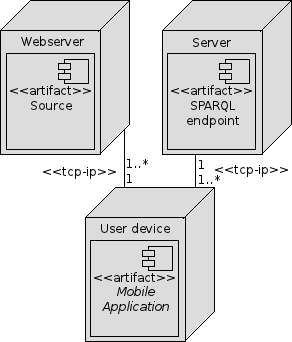
\includegraphics{./figures/deployment-m.png}
 \caption{Diagram nasazení mobilní aplikace}
 \label{fig:mobile:deployment}
\end{figure}


\subsection{Návrh řešení}
Návrh (\textit{design}) byl prováděn po rozvržení architektury, za přispění volby použitých technologií a reflektovány do něj byly i požadavky na uživatelské rozhraní.

Systém byl rozdělen do čtyř modulů sloužících jako průvodce, navigace, \glsname{SPARQL} konzole a nápověda. Každý z modulů je víceméně nezávislý na těch ostatních, jen nástroje pro dotazování se \glsname{SPARQL} endpointu byly vyčleněny pro možnost využití ve všech modulech.

Na obrázku \ref{fig:mobile:class} je znázorněn třídní diagram (\textit{class diagram}) mobilní aplikace.

\begin{figure}[h]
 \centering
 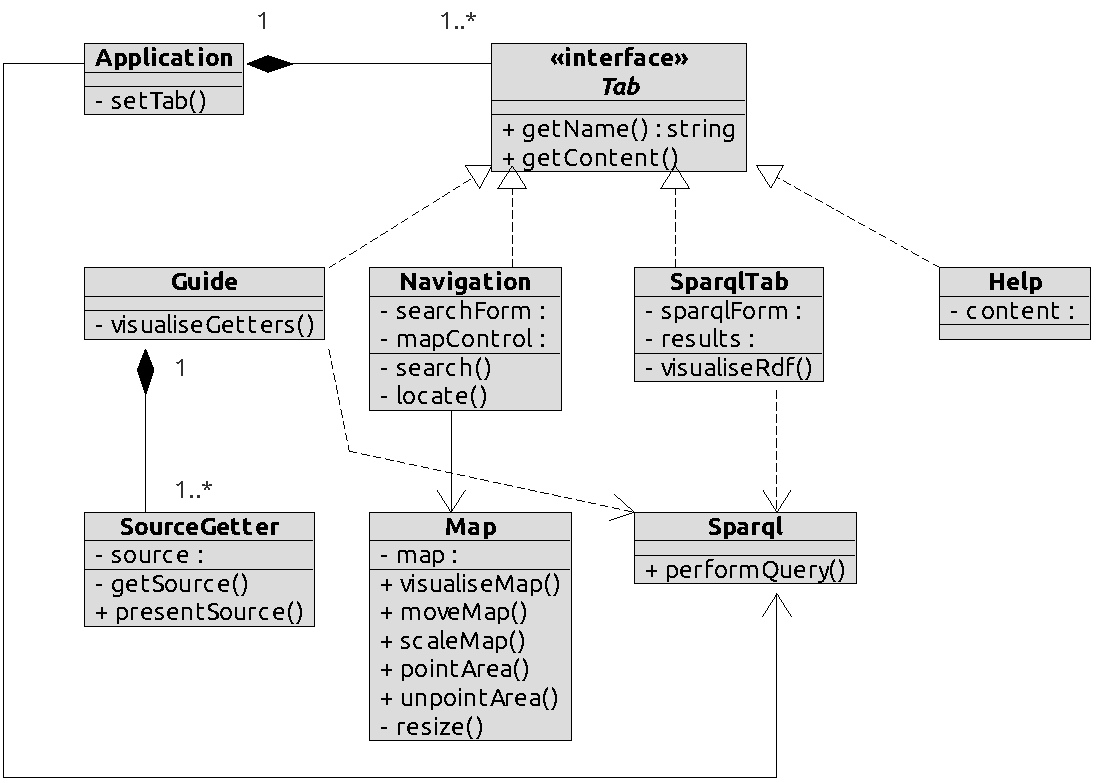
\includegraphics[width=14.30cm]{./figures/class-m.pdf}
 % class-m.png: 535x376 pixel, 95dpi, 14.30x10.05 cm, bb=0 0 405 285
 \caption{Třídní diagram mobilní aplikace}
 \label{fig:mobile:class}
\end{figure}

% \subsubsection{Získávání dat ze zdrojů}
% V rámci aplikace je nutné získávat data z jiných zdrojů: \glsname{SPARQL} endpointu serverové aplikace, ale i přímo z oficiálních zdrojů fakulty.
% \subsubsection{Vyhledávání }
% \subsubsection{Navigace}


\subsection{Návrh bezpečnosti}
Návrh aplikace je poměrně přímočarý a není ho třeba nějak složitě vysvětlovat, co se ale týče bezpečnosti, je to podstatně horší -- v prováděných činnostech se vyskytuje několik skrytých hrozeb, které je třeba identifikovat a odstranit z nich plynoucí zranitelnosti.

\subsubsection{Dekompozice}
Byly identifikovány následující komponenty:
\begin{itemize}
 \item Mobilní aplikace.
 \item \glsname{SPARQL} endpoint.
 \item Zdroje informací.
 \item Uživatel.
\end{itemize}
Plná důvěra může být pouze v rámci mobilní aplikace -- tam, kde nemůže být žádný zásah zvenčí. Dále lze do určité míry důvěřovat \glsname{SPARQL} endpointu -- bude provozován pod vlastní správou. Zdroje informací a vstupy uživatele jsou naopak nedůvěryhodné -- jsou plně v režii třetích stran. Hranice důvěry jsou přesto mezi všemi komponentami.

\subsubsection{Identifikace hrozeb}
Hrozby je třeba identifikovat pouze na komponentě \emph{mobilní aplikace}, ostatní komponenty jsou v tuto chvíli irelevantní:
\begin{itemize}
 \item Podvržení nepravdivých dat.
 \item Podvržení škodlivých dat.
\end{itemize}

\subsubsection{Identifikace zranitelností}
Obě výše uvedené hrozby mohou vyústit ve zranitelnosti. S podvržením nepravdivých dat se bohužel nevypořádáme - data jsou čerpána z oficiálních zdrojů a v případě, že někdo kompromituje je, nám žádné z opatření nepomůže. Zranitelnosti plynoucí z druhé hrozby omezil ale lze. Mohou jimi být:
\begin{itemize}
 \item Injektáž škodlivého skriptu ze zdroje -- vzhledem k použitým technologiím, JavaScriptu.
 \item Injektáž škodlivého značkovacího kódu ze zdroje -- neuzavřené \glsname{HTML} elementy, identifikátory duplicitní k již existujícím, destruktivní formátování\dots
 \item Neošetřený uživatelský vstup -- neplatný regulární výraz\dots
%  \item Pozměnění komunikace se serverem mimo uživatelovy privilegia.
\end{itemize}

\subsubsection{Důsledky}
\begin{itemize}
 \item Je třeba ve výchozím nastavení zakázat všechny cizí vstupy a potřebným udělit výjimky.
 \item Je třeba důsledně ošetřovat vstupy.
 \item Je třeba zamezit injektování cizích JavaScriptů.
 \item Je třeba ve výchozím nastavení zakázat všechny HTML elementy cizích zdrojů a potřebným udělit výjimky.
 \item Je třeba ve výchozím nastavení zakázat všechny HTML atributy cizích zdrojů a potřebným udělit výjimky.
 \item Je třeba ve výchozím nastavení zakázat všechny hodnoty HTML atributů cizích zdrojů a potřebným udělit výjimky.
\end{itemize}


\subsection{Návrh uživatelského rozhraní}
\todo{Pojednání o vytvořených prototypech, možná nakonec pod něco zařadím, nebude mít velký rozsah.}
% Po ujasnění několika základních potřeb a požadavků jsem začal vytvářet prototypy. Nejprve pouze jednoduché low fidelity prototypy pro vyjasnění základních požadavků, později sofistikovanější high fidelity prototypy reprezentující chování i vzhled výsledné aplikace.
% 
% \subsection{Low fidelity prototypy}
% Low fidelity prototypy jsou, většinou papírové, snadno vytvořitelné prototypy, na kterých se navrhují a testují některé základní aspekty aplikace -- rozvržení komponent, jednoduchá interakce, návaznost akcí a podobně. Mají tu výhodu, že zadavateli přiblíží finální aplikaci, udělá si konkrétnější představu a lépe se mu pak formulují požadavky.
% 
% Za pomoci low fidelity prototypů se vymezily jednotlivé obrazovky aplikace. Výchozí obrazovka je v podstatě jedinou nutnou obrazovkou aplikace, obsahuje menu pro přechod do dalších obrazovek, vyhledávací formulář a krátkou nápovědu. Dalšími obrazovkami jsou nápověda, nápověda regulárních výrazů a obrazovka se základními informacemi o programu.
% 
% Nejvýznamnějším ovládacím prvkem bude velké vyhledávací pole uprostřed úvodní obrazovky -- uživatel zde bude moci zadat všechno, co potřebuje nalézt, a aplikace by mu to měla vyhledat. V případě, že bude nalezeno více výsledků, zobrazí se jejich seznam (viz obrázek~\ref{fig:LFviceVysledku}\footnote{Low fidelity prototypy byly vytvořeny v nástroji Balsamiq Mockups \cite{BalsamiqMockups}.}), ze kterého si bude moci uživatel vybrat nebo upřesnit hledaný výraz, jinak se navede rovnou k cíli (viz obrázek~\ref{fig:LFjedinyVysledek}).
% 
% \begin{figure}[ht]
% \begin{center}
% 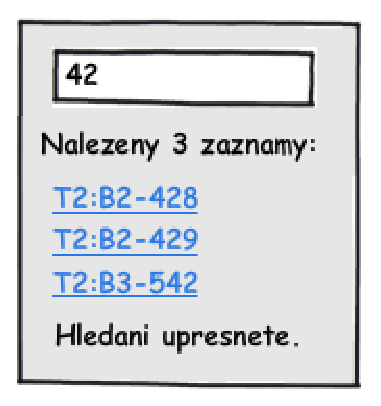
\includegraphics[width=30mm]{figures/LFviceVysledku}
% \caption{Nalezení několika výsledků}
% \label{fig:LFviceVysledku}
% \end{center}
% \end{figure}
% 
% \begin{figure}[ht]
% \begin{center}
% 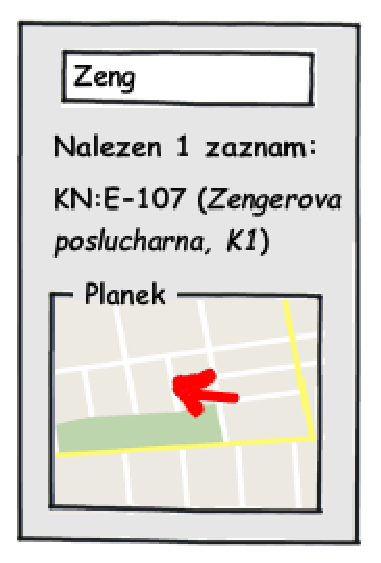
\includegraphics[width=30mm]{figures/LFjedinyVysledek}
% \caption{Nalezení jediného výsledku}
% \label{fig:LFjedinyVysledek}
% \end{center}
% \end{figure}
% 
% Aplikace by ještě měla poskytovat rozšířené vyhledávání s upřesněním hledaných míst a~zadáním výchozího bodu.
% 
% \noindent\textbf{Ostatní low fidelity prototypy jsou na přiloženém CD.}
% 
% 
% 
% \subsection{High fidelit prototyp}
% High fidelity prototypy jsou už sofistikovanějšími prototypy, jejich vytvoření tudíž trvá déle, ale přesto se je vyplatí udělat před finální aplikací -- nemají totiž plnou funkčnost konečné aplikace, nemusí ošetřovat vstupy a řešit nestandardní situace, takže se pořád vytvoří relativně rychle, přičemž už zadavateli dokáží realisticky demonstrovat finální práci s aplikací.
% 
% High fidelity prototyp jsem vytvořil pomocí XHTML, ECMAScriptu a CSS. Jedná se o~velmi vhodné technologie pro tvorbu prototypů -- rychle se vytvoří a snadno se pak upravují. Testování takto vytvořených prototypů je také příjemné -- v případě v prototypu nevyřešené situace lze snadno připravit výslednou situaci a testerovi ji na dálku bez nějakých komplikací podstrčit.
% 
% Na obrázku \ref{fig:HFviceVysledku} je vidět high fidelity prototyp ve stavu zobrazení více výsledků vyhledání.
% 
% \begin{figure}[ht]
% \begin{center}
% 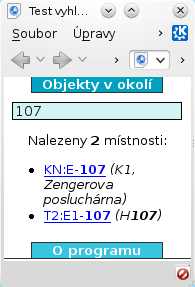
\includegraphics[width=30mm]{figures/HFviceVysledku}
% \caption{Nalezení několika výsledku}
% \label{fig:HFviceVysledku}
% \end{center}
% \end{figure}
% 
% Testování high fidelity prototypů je hlouběji popisované v kapitole o testování (viz \ref{sec:testhfp}).
% 
% \noindent\textbf{High fidelity prototyp je na přiloženém CD.}



\subsection{Použité technologie}
Níže uvádím soupis použitých technologií s odůvodněním, proč byly vybrány a v jakém kontextu použity.

\subsubsection{HTML5}
Většina technologií tvořících mobilní aplikaci by se dala zahrnout do pojmu HTML5 (v širším smyslu významu). Pomocí JavaScriptu se manipuluje s \glsname{HTML} strukturou, která je prezentována za pomocí \glsname{CSS}, klíčová část aplikace -- mapa -- je tvořena \glsname{SVG} (o tom ještě dále). Technologie byly vybrány pro jejich výbornou portovatelnost -- téměř všechna dnešní zařízení je implementují podobně (nebo alespoň mají takové výkonnostní parametry, že na nich lze provozovat přidanou vrstvu abstrahující od skutečné implementace).

\subsubsection{SVG}
Mapa použitá v aplikaci je implementována prostřednictvím \glsname{SVG}. Rozhodnutí bylo učiněno na základě identifikace a porovnání možných technologií:
\begin{itemize}
 \item Statické obrázky s předgenerovanými proměnnými částmi.
 \item Statické obrázky s dynamicky pozicovanými proměnnými částmi.
 \item Dynamicky kreslené obrázky na \textit{canvas}.
 \item Statické \glsname{SVG} s dynamickými úpravami.
\end{itemize}

První zmíněné řešení bylo zavrženo kvůli nízké flexibilitě -- není možné dopředu vygenerovat všechny varianty obrázků, které by pokrývaly možné situace -- i kdyby to možné bylo, množství obrázků by bylo velmi vysoké\footnote{Pro pokrytí všech situací by byly třeba zvlášť obrázky s vyznačením kterékoliv místnosti, kteréhokoliv bodu zájmu, kterékoliv výchozí pozice\dots Vzhledem k rozsáhlosti mapy by tak počet obrázků byl enormní.} a pro omezenou paměťovou kapacitu cílových zařízení nevhodné.

Druhý přístup, dynamické pozicování, byl zavržen z důvodů optimalizací rozvržení prvků mobilními prohlížeči -- není zaručené, že se prvek (například ukazatel nalezené místnosti) skutečně umístí, kam má.

Nová vlastnost HTML5, kreslení prostřednictvím JavaScriptu na \textit{canvas} element, byla, narozdíl od předchozích možností, zvažována až do finálního rozhodnutí -- ačkoliv se jedná o řešení čistě v režii již používaných technologií (JavaScript, HTML), jeho využití jsem z několika důvodů zavrhl:
\begin{itemize}
 \item Neumožňuje nakreslený obrázek nijak upravit (například posunout ukazatel na mapě), ale musí se vždy překreslit, což je náročnější na zdroje.
 \item Kvůli principu dynamického generovaní obrázků JavaScriptem nelze kostru připravit pomocí běžných grafických editorů.
 \item Subjektivně mi přijde práce s mapou jako \glsname{SVG} obrázkem reprezentovaným \glsname{XML} dokumentem majícím \glsname{DOM} přehlednější, než s méně strukturovatelným JavaScriptem.
\end{itemize}

Reprezentaci mapy jsem tedy svěřil \glsname{SVG} z následujících důvodů:
\begin{itemize}
 \item Snadné vytvoření mapy prostřednictvím běžného grafického editoru.
 \item Možnost znovupoužití mapy standardního grafického formátu i v jiných projektech.
 \item Práce s mapou (něpř. vyznačování pozic) se provádí pouhodou úpravou jejího \glsname{DOM}.
 \item I po úpravách se stále jedná o týž objekt -- není nutné ho překreslovat.
\end{itemize}

Nutno podotknout, že jsou implementace kreslení na \textit{canvas} a \glsname{SVG} na různých mobilních zařízeních na různých úrovních, ani jedna ovšem nemá výrazně navrch \cite{CanIUse} \cite{MobileHtml}.

\subsubsection{PHP}
Z důvodů popsaných v podsekci \ref{sec:mobil:cross-origin} na straně \pageref{sec:mobil:cross-origin} bylo nutné vytvořit podpůrnou serverovou aplikaci -- proxy. Po úvaze jsem se rozhodl pro využití jazyka \glsname{PHP}, který je podporovaný jako jediný nástroj pro tvorbu dynmického obsahu na fakultním webovém serveru \url{http://webdev.fit.cvut.cz/}. Tuto kombinaci, vzhledem k její podpoře ze strany fakulty a určení práce pro fakulní nasazení, považuji i přes jinde využitý JavaScript za vhodnou.


\subsection{Použité knihovny}
V práci byla, po úvaze, nakonec využita i práce třetích stran -- svobodné knihovny \emph{jQuery} a \emph{HTML Purifier}. Jejich krátký popis a odůvodnění následují:

\subsubsection{jQuery}
A

\subsubsection{HTML Purifier}
Po několika vlastních implementacích nástroje na pročištění a ošetření \glsname{HTML} vstupů pocházejících od třetích stran jsem sáhl k implementaci již prověřené -- oblast ošetření aplikace před škodlivými vstupy má z hlediska bezpečnosti vysokou prioritu a neustále se objevující nové hrozby nakonec vedly k tomu, že jsem se rozhodl nespoléhat na své vlastní implementace a využít \textit{know-how} tvůrců svobodné \glsname{PHP} knihovny  HTML Purifier (\url{http://htmlpurifier.org/}) -- ta odstraní případná nebezpečí za využití pokročilého auditovaného \textit{whitelistu} a v případě potřeby navíc zajistí validitu kódu. Knihovna je využita v rámci proxy zmíněné v předchozím odstavci.


\subsection{Použité nástroje}
Pro tvorbu aplikace byly použity převážně následující nástroje. Majorita jich je uvolněných pod svobodmými licencemi, zpravidla \glsname{GNU} \glsname{GPL} nebo kompatibilními. Jedinou výjimkou jsou některé mobilní prohlížeče, které byly použity k testování aplikace.

\subsubsection{Kate}
Textový editor \glsname{Kate} (\url{http://kate-editor.org/}) byl, mimo serverové (viz část \ref{sec:server:tools:kate} na straně \pageref{sec:server:tools:kate}), vybrán i pro tvorbu mobilní aplikace. Nástroj byl zvolen na základě již dříve zmíněných důvodů pro napsání kódu v JavaScriptu, \gls{HTML}, \gls{CSS} i úpravy mapy v \gls{SVG}.

\subsubsection{Inkscape}
Grafické podklady práce byly vytvořeny v editoru vektorové grafiky Inkscape (\url{http://www.inkscape.org/}). Nástroj implementuje téměř kompletní specifikaci formátu \glsname{SVG} verze 1.1, je multiplatformní a svobodný. Inkscape byl vybrán kvůli předchozím výborným zkušenostem s prací v něm a celkové vhodnosti pro tvorbu mapových podkladů.

\subsubsection{Kompare}
Nástroj byl zvolen ze stejných důvodů, jak tomu bylo u serverové aplikace (viz část \ref{sec:server:tools:kompare} na straně \ref{sec:server:tools:kompare}).

\subsubsection{Webové prohlížeče}
Pro správné odlazení aplikací, průzkum možností a testování byly vybrány následující prohlížeče. Některé kvůli jejich významnému zastoupení mezi uživateli, jiné pro odlazení aplikace i v jiných implementacích použitých technologií.
\begin{itemize}
 \item Mozilla Firefox (\url{http://www.mozilla.org/firefox}).
 \item Chromium (\url{http://chromium.org/}).
 \item rekonq (\url{http://rekonq.kde.org/}).
 \item Prohlížeč platformy Android (\url{http://www.android.com/}) -- verze 2 a 4.
 \item Opera Mobile (\url{http://www.opera.com/mobile}).
 \item Internet Explorer Mobile (\url{http://www.microsoft.com/windowsphone/en-us/features/default.aspx#internet-explorer}).
Mimo výše uvedených navíc nabídl pan inženýr Havryluk, vedoucí práce, otestování v následujících prohlížečích:
 \item Google Chrome for Android (\url{https://www.google.com/intl/en/chrome/android/}).
 \item Prohlížeč platformy Android (\url{http://www.android.com/}) -- verze 3.
 \item Dolphin Browser (\url{http://dolphin-browser.com/}).
 \item Nokia Browser for Symbian  (\url{http://browser.nokia.com/}).
 \item Prohlížeč platformy BlackBerry (\url{http://us.blackberry.com/smartphones/features/internet.jsp}).
 \item Safari (\url{http://www.apple.com/safari/}).
\end{itemize}

\subsubsection{Git}
Nástroj byl zvolen ze stejných důvodů, jak tomu bylo u serverové aplikace (viz část \ref{sec:server:tools:git} na straně \ref{sec:server:tools:git}).
